\section{Method}
\label{sect:method}

This section presents our unsupervised method for TF design, enabling semi-automated material classification and initial TF specification for intuitive volume exploration.

Fig.~\ref{fig:volume-exploration-pipeline} shows an overview. After organizing the dataset into a volume grid, we apply three steps: dimensionality reduction, clustering, and pivot-based indexing.

\begin{figure*}[htb!]
    \centering
    \caption{Overview of the proposed unsupervised method for transfer function definition and design.}
    \label{fig:volume-exploration-pipeline}
    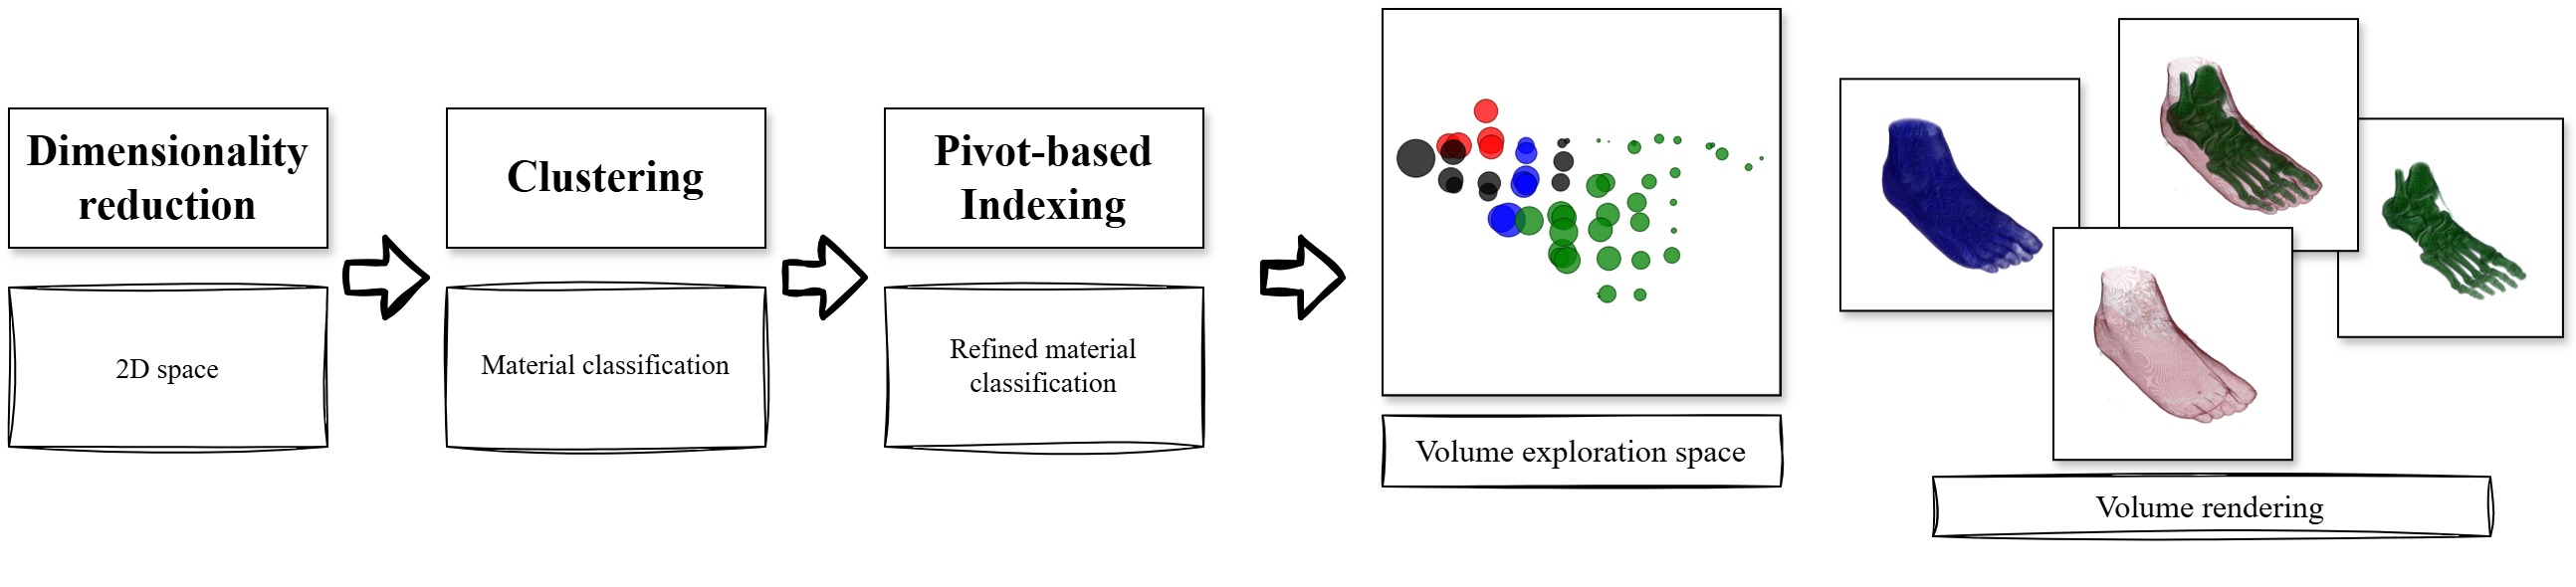
\includegraphics[width=\textwidth]{figs/method-overview.jpg}
\end{figure*}

\subsection{Dimensionality Reduction}
\label{subsect:feature-extraction}

We use FastMap~\cite{faloutsos1995} to project high-dimensional data into 2D while preserving clustering structure. The algorithm finds two distant pivots and projects points onto the line between them.

Let $d$ be the number of attributes and $n$ the number of voxels. The steps are:
\begin{enumerate}
    \item Find two points (pivots) furthest apart.
    \item Project points onto a hyperplane orthogonal to the pivots’ line.
\end{enumerate}

To avoid quadratic complexity, we use the heuristic from~\cite{faloutsos1995} (Algorithm~\ref{alg:pivot-searching-of-fastmap}) which approximates distant pivots.

\begin{algorithm}
    \caption{Pivot searching of FastMap.}
    \label{alg:pivot-searching-of-fastmap}
    \KwIn{$\mathbb{O}$}
    \KwOut{Pivots $O_a$, $O_b$}
    $O_a \gets$ random point $o \in \mathbb{O}$\\
    $O_b \gets$ point $o \in \mathbb{O}$ farthest from $O_a$\\
    $O_a \gets$ point $o \in \mathbb{O}$ farthest from $O_b$
\end{algorithm}

Time complexity is $\mathcal{O}(nk)$ with $k=2$.

\subsection{Clustering}
\label{subsect:clustering}
A major goal of our method is to simplify material classification and facilitate the highlighting of volume details. We address this objective by employing a classical density-based clustering algorithm, the DBSCAN~\cite{ester1996}. 

DBSCAN is a widely utilized algorithm known for its success across various applications~\cite{schubert2017}. Nevertheless, its adoption in DVR comes with some caveats.  The original version~\cite{ester1996} exhibits a time complexity of $\mathcal{O} (n^2)$ in the worst case~\cite{schubert2017}. With practical usability in mind, we implemented a grid-based  DBSCAN proposed by \cite{gunawan2013}. This version claims a time complexity of $\mathcal{O} (n \log (n))$. 

Like the original algorithm~\cite{ester1996}, the 2D grid version also has $minPts$ and $\varepsilon$ as input parameters. In this way, the user must fine-tune such parameters to best classify the volume data. 

When this method step ends, each cluster comprises a subset of voxels that potentially represent a region of interest.

\cite{gunawan2013} introduces the concept of a grid to improve the efficiency of the clustering process, especially for high-dimensional datasets. The authors improve the scalability and efficiency of traditional DBSCAN by leveraging grid-based partitioning and density estimation techniques. Detailed explanations are provided in the works of \cite{gunawan2013} and \cite{gan2015}. The algorithm operates on a cell grid and comprises the tasks summarized next.

\begin{enumerate}
    \item Grid partitioning. The first step involves partitioning the space into a grid of cells. Each cell represents a small portion of the entire space.

    \item Density estimation. Within each cell, the algorithm calculates the density of points. The density is usually estimated using a distance threshold ($\varepsilon$) to determine the neighborhood of each point.

    \item Identifying core points. Points with a density above a certain threshold ($minPts$) are considered core points. These core points are potential seeds for clusters.

    \item Expanding clusters. Starting from a core point, the algorithm expands the cluster by iteratively adding neighboring points that also qualify as core points. The expansion continues until there are no more core points to be added.

    \item Handling border points. Points that are within the $\varepsilon$ neighborhood of a core point but do not meet the density requirement to be considered core themselves are classified as border points. Border points are assigned to the cluster of their nearest core point.

    \item Handling noise. The points that are not core and do not belong to any cluster are considered noise points.
\end{enumerate}

\subsection{Pivot-based indexing}
\label{subsect:pivot-based-indexing}

To reduce scatter plot clutter, we plot only selected pivots within each cluster. Each cluster is subdivided into sub-clusters by assigning points to their nearest pivot (Algorithm~\ref{alg:subclustering-finding}).

\begin{algorithm}
    \caption{Finding sub-clusters within a cluster.}
    \label{alg:subclustering-finding}
    \KwIn{Points $\mathbb{P}$ of cluster $c$}
    \KwIn{Pivots $\mathbb{P}_s$ of cluster $c$}
    \KwOut{Points with sub-cluster assignment}
    \ForEach{$p \in \mathbb{P}$}{
        $p_s \gets$ nearest pivot in $\mathbb{P}_s$ \\
        Assign $p$ to $p_s$'s sub-cluster
    }
\end{algorithm}

We select pivots using Sparse Spatial Selection (SSS)~\cite{pedreira2007}, which adds points as pivots if they are sufficiently distant from existing ones, controlled by a distance factor $\alpha$.

\begin{algorithm}
    \caption{Sparse Spatial Selection.}
    \label{alg:sss}
    \KwIn{Points $\mathbb{P}$}
    \KwOut{Selected pivots $\mathbb{P}_s$}
    $\mathbb{P}_s \gets \{p_1\}$ \\
    \ForEach{$p \in \mathbb{P}$}{
        \If{$\forall p_s \in \mathbb{P}_s, \text{dist}(p, p_s) \geq M\alpha$}{
            $\mathbb{P}_s \gets \mathbb{P}_s \cup \{p\}$
        }
    }
\end{algorithm}

Adjusting $\alpha$ controls the number of pivots: smaller $\alpha$ selects more pivots; values near $1$ select fewer.

